\documentclass[a4paper, 12pt]{article}
\usepackage[top=1cm, bottom=2.1cm, left=2cm, right=2cm]{geometry}
\usepackage[utf8]{inputenc}
\usepackage{graphicx, caption}
\usepackage{float}
\usepackage{amsmath, amsfonts, amssymb, esint}
\usepackage{color}
\usepackage{hyperref}
\usepackage{multicol}
\usepackage{wallpaper}

\CenterWallPaper{1}{./img/background.png}

\hypersetup{
    colorlinks=true,
    linkcolor=blue,
    filecolor=magenta,      
    urlcolor=cyan,
}

\definecolor{red}{rgb}{1,0,0}
\newcommand{\red}[1]{\textcolor{red}{#1}}

\newcommand{\cabecalho}[4]
{
	\begin{figure}
		\centering
		\href{https://ligaolimpicadeastronomia.com.br/}{
\includegraphics[scale=0.6]{./img/logos.png}}
	\end{figure}
	
	\begin{center}
		\begin{large}
			\textbf{#1}	
		\end{large}
			\linebreak Listas OBA (Nível 4) -- #2ª Lista
			\linebreak #3
		\end{center}
	
	\begin{flushright}
		Material elaborado por \textbf{#4}
	\end{flushright}
}

\begin{document}
	\cabecalho{\red{Gabarito}}{3}{Fotometria \& Estrelas}{Iago Braz Mendes}
	
	\begin{flushleft}
	\begin{itemize}
		\item \textbf{Questão 1) (1 ponto)} A nossa estrela -- o Sol -- possui 6 camadas, 3 internas e 3 externas. Observe a seguinte representação com números de $1$ a $6$ em cada camada solar:
			\begin{figure}[H]
				\centering
				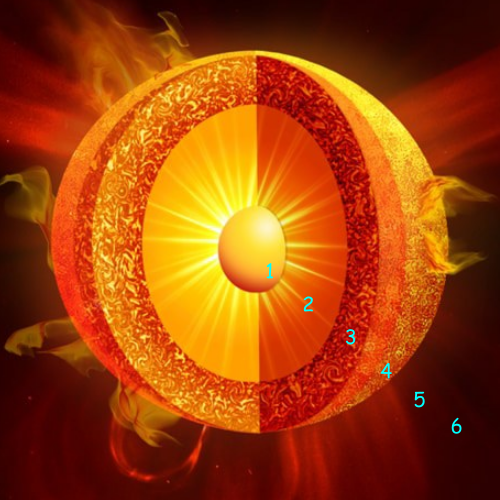
\includegraphics[scale=0.6]{./img/1.png}
			\end{figure}
			\begin{itemize}
				\item \textbf{Pergunta 1a) (0,6 ponto) (0,1 cada acerto)} Abaixo, os 6 nomes das camadas solares estão em ordem aleatória. Insira o número correspondente ao representado na imagem.
					\begin{multicols}{2} \begin{itemize}
						\item[$(\red{3})$] Zona convectiva
						\item[$(\red{6})$] Coroa
						\item[$(\red{4})$] Fotosfera
						\item[$(\red{1})$] Núcleo
						\item[$(\red{2})$] Zona radiativa
						\item[$(\red{5})$] Cromosfera
					\end{itemize} \end{multicols}
				\item \textbf{Pergunta 1b) (0,1 ponto)} Quais as formas de transmissão de calor nas camadas $2$ e $3$, respectivamente?
					\begin{itemize}
						\item[$(\quad)$] Condução e Radiação
						\item[$(\red{X})$] Radiação e Convecção
						\item[$(\quad)$] Convecção e Condução
						\item[$(\quad)$] Convecção e Radiação
					\end{itemize}
				\item \textbf{Pergunta 1c) (0,3 ponto)} Algo que ainda intriga vários cientistas é o fato de a camada $6$ possuir uma maior temperatura do que as camadas $4$ e $5$. O fator responsável por essa peculiaridade mais aceito atualmente também causa irregularidades na atmosfera solar, como os ventos solares. Qual é esse fator?
					\begin{itemize}
						\item[$(\quad)$] Equilíbrio entre força gravitacional e a pressão de radiação
						\item[$(\quad)$] Escapamento de neutrinos originados pelas reações nucleares
						\item[$(\quad)$] Movimento do Sol ao redor do baricentro do Sistema Solar
						\item[$(\red{X})$] Variação dos campos magnéticos
					\end{itemize}
			\end{itemize}
		\item \textbf{Questão 2) (1 ponto)} A energia proveniente do Sol é originada por meio do ciclo p-p, o qual pode ser simplificado para a seguinte reação nuclear:
			$$H_1^2 + H_1^3 \longrightarrow He_2^4 + n_0^1 + \gamma$$
			em que $H_1^2$ (deutério) e $H_1^3$ (trítio) são alótropos do hidrogênio, $He_2^4$ é um âtomo de hélio, $n_0^1$ é um nêutron, e $\gamma$ representa a energia liberada. \linebreak
			As massas atômicas envolvidas nessa reação são dadas a seguir:
				\begin{multicols}{2} \begin{itemize}
					\item[$>$] $m(H_1^2) \simeq 2,014 \; uma$
					\item[$>$] $m(H_1^3) \simeq 3,016 \; uma$
					\item[$>$] $m(He_2^4) \simeq 4,003 \; uma$
					\item[$>$] $m(n_0^1) \simeq 1,009 \; uma$
				\end{itemize} \end{multicols}
				\begin{itemize}
					\item \textbf{Pergunta 2a) (0,4 ponto)} Calcule a taxa de massa perdida ($t$), em porcentagem, usando a reação nuclear passada. \linebreak
						\textbf{Dica:} $t= \left| \frac{m'-m_0}{m_0} \right|$, em que $m_0$ e $m'$ são as massas antes e depois da reação, respectivamente.
						\red{\begin{itemize}
							\item Primeiramente, precisamos calcular $m_0$ e $m'$:
								$$m_0 = m(H_1^2) + m(H_1^3) = 2,014 + 3,016 = 5,030 \; uma$$
								$$m' = m(He_2^4) + m(n_0^1) = 4,003 + 1,009 = 5,012 \; uma$$
							\item Assim, a variação de massa é:
								$$\Delta m = m' - m_0 = 5,012 - 5,030 = - 0,018 \; uma$$
							\item Finalmente, temos:
								$$t = \left| \frac{\Delta m}{m_0} \right| = \left| - \frac{0,018}{5,030} \right|$$
								$$\therefore \quad t \simeq 0,004 = 0,4\%$$
						\end{itemize}}
						\textbf{Resposta 2a)}: $\red{0,4\%}$
					\item \textbf{Pergunta 2b) (0,3 ponto)} Considerando que toda a massa do Sol seja composta por alótropos de hidrogênio e que o ciclo p-p é a única reação nuclear que ocorre até a tais alótropos se esgotarem, qual será a massa convertida em energia, em $kg$? \linebreak
						\textbf{Dados:} $M_{Sol} \simeq 2 \cdot 10^{30} \; kg$
						\red{\begin{itemize}
							\item Basta multiplicar $M_{Sol}$ por $t$:
								$$m = M_{Sol} \cdot t = 2 \cdot 10^{30} \cdot 4 \cdot 10^{-3}$$
								$$\therefore \quad m = 8 \cdot 10^{27} \; kg$$
						\end{itemize}}
						\textbf{Resposta 2b)}: $\red{8 \cdot 10^{27} \; kg}$
					\item \textbf{Pergunta 2c) (0,3 ponto)} Qual a quantidade de energia gerada pela massa calculada no item anterior? \linebreak
						\textbf{Dica:} $E = m c^2$
						\red{\begin{itemize}
							\item Sabendo que $c=3 \cdot 10^8 \; \frac{m}{s}$, temos:
								$$E = m \cdot c^2 = 8 \cdot 10^{27} \cdot (3 \cdot 10^8)^2$$
								$$\therefore \quad E = 7,2 \cdot 10^{43} \approx 7 \cdot 10^{43} \; J$$
						\end{itemize}}
						\textbf{Resposta 2c)}: $\red{7 \cdot 10^{43} \; J}$
				\end{itemize}
				
		\item \textbf{Questão 3) (1 ponto)} Na Astronomia, os conceitos de Luminosidade e Fluxo são frequentemente usados e, portanto, é importante saber diferenciá-los. Observe o esquema seguinte representando a emissão de energia do Sol:
			\begin{figure}[H]
				\centering
				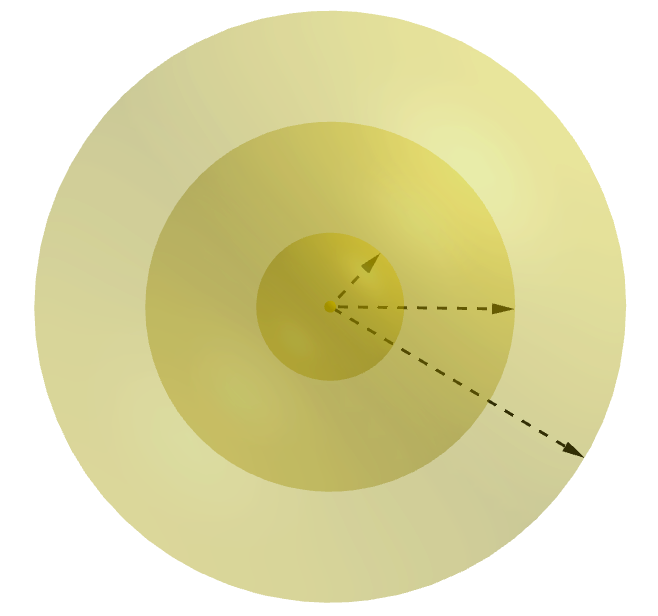
\includegraphics[scale=0.45]{./img/3.png}
			\end{figure}
			Como você pode perceber, o ``brilho" é reduzido à medida que a distância da fonte luminosa aumenta. Contudo, a energia emitida deve ser a mesma, visto que não se pode perder energia no universo. \linebreak
			Nesse contexto, precisamos fazer duas definições:
				\begin{enumerate}
					\item \textit{Luminosidade:} é a quantidade de energia emitida a cada unidade de tempo (potência) e a sua unidade no S.I. é o watt $\left( W=\frac{J}{s} \right)$
					\item \textit{Fluxo:} é a quantidade de potência recebida a cada unidade de área e a sua unidade no S.I. é watt por metro quadrado $\left( \frac{W}{m^2} \right)$
				\end{enumerate}
			Dito isso, é possível analisar que os melhores termos para ``brilho" e ``energia emitida" seriam \textit{fluxo} e \textit{luminosidade}, respectivamente. Como já discutimos, a luminosidade deve se manter constante na superfície da esfera luminosa emitida e o fluxo é inversamente proporcional à distância da fonte luminosa. Para encontrarmos uma fórmula que descreva essas quantidades, basta inserirmos a área superficial dessa esfera ($A=4 \pi r^2$):
				$$F = \frac{L}{4 \pi r^2}$$
			em que $F$ é o fluxo, $L$ é a luminosidade, e $r$ é a distância à fonte (raio da esfera luminosa).
			\begin{itemize}
				\item \textbf{Pergunta 3a) (0,5 ponto)} A distância entre a Terra e o Sol é $1 \; UA \approx 1,5 \cdot 10^{11} \; m$. Sabendo disso e que $L_{Sol} \simeq 3,8 \cdot 10^{26} \; W$, determine o fluxo solar que recebemos. \linebreak
					\textbf{Dica:} para facilitar as contas, considere $\pi \approx 3$
					\red{\begin{itemize}
						\item Aplicando os valores na fórmula do fluxo, temos:
							$$F_{Sol} = \frac{L_{Sol}}{4 \pi r^2} = \frac{3,8 \cdot 10^{26}}{4 \cdot 3 \cdot (1,5 \cdot 10^{11})^2}$$
							$$\therefore \quad F_{Sol} \simeq 1,4 \cdot 10^3 \; \frac{W}{m^2} = 1400 \; \frac{W}{m^2}$$
					\end{itemize}}
					\textbf{Resposta 3a)}: $\red{1400 \; \frac{W}{m^2}}$
				\item \textbf{Pergunta 3b) (0,5 ponto)} O fluxo da estrela Sirius -- alfa da constelação Cão Maior -- recebido na Terra é $F_{Sirius} \simeq 1,2 \cdot 10^{-7} \; \frac{W}{m^2}$ e a sua luminosidade é $L_{Sirius} \simeq 9,7 \cdot 10^{27}$. Se a Terra estivesse a uma mesma distância do Sol e de Sirius, qual estrela possuiria o maior fluxo?
					\red{\begin{itemize}
						\item Se as 2 estrelas estivessem a uma mesma distância do da Terra, teríamos a seguinte razão:
							$$\frac{F_{Sirius}}{F_{Sol}} = \frac{L_{Sirius}}{4 \pi r^2} \frac{4 \pi r^2}{L_{Sol}} = \frac{L_{Sirius}}{L_{Sol}}$$
						\item Como $L_{Sirius} > L_{Sol}$, temos que $F_{Sirius} > F_{Sol}$.
					\end{itemize}}
					\begin{itemize}
						\item[$(\quad)$] Sol
						\item[$(\red{X})$] Sirius
						\item[$(\quad)$] As duas estrelas teriam o mesmo fluxo
						\item[$(\quad)$] Impossível de determinar com as informações passadas
					\end{itemize}
			\end{itemize}
			
		\item \textbf{Questão 4) (1 ponto)} A luminosidade das estrelas depende tanto em seu tamanho quanto em sua temperatura. Nesse sentido, podemos usar a Lei de Stefan-Boltzmann para mostrar matematicamente essa relação:
			$$L=4 \pi R^2 \sigma T^4$$
			em que $L$ é a luminosidade, $R$ é o raio, $T$ é a temperatura, e $\sigma$ é a constante de Stefan-Boltzmann $\left( \sigma \simeq 5,67 \cdot 10^{-8} \; \frac{W}{m^2K^4} \right)$. \linebreak \linebreak
			Mais importante do que memorizar essa equação, é preciso entender que a luminosidade é diretamente proporcional ao raio ao quadrado e à temperatura elevada à quarta pontência. Matematicamente, temos:
				$$L \propto R^2 T^4$$
			Além disso, podemos determinar a cor de uma estrela a partir de sua temperatura (e vice-versa). Para tanto, precisamos utilizar a Lei de Wien:
				$$\lambda T = b$$
				em que $\lambda$ é o comprimento de onda em que a maior quantidade de energia é emitida, $T$ é a temperatura, e $b$ é a constante de Wien ($b \simeq 2,90 \cdot 10^{-3} \; mK$). \linebreak \linebreak
				\begin{itemize}
					\item \textbf{Pergunta 4a) (0,1 ponto)} Se o raio de uma estrela for reduzido pela metade $\left( R'=\frac{R_0}{2} \right)$ e sua temperatura for multiplicada por 2 ($T'=2T_0$), o que acontecerá com a luminosidade?
						\red{\begin{itemize}
							\item Usando a Lei de Stefan-Boltzmann, temos:
								$$\frac{L'}{L_0} = \frac{4 \pi R'^2 \sigma T'^4}{4 \pi R_0^2 \sigma T_0^4} = \left( \frac{R'}{R_0} \right)^2 \cdot \left( \frac{T'}{T_0} \right)^4$$
								$$\therefore \quad \frac{L'}{L_0} = \left( \frac{1}{2} \right)^2 \cdot 2^4 = 2^2 = 4$$
								$$\therefore \quad L' = 4 L_0$$
						\end{itemize}}
						\begin{itemize}
							\item[$(\quad)$] $L'=L_0$
							\item[$(\quad)$] $L'=2L_0$
							\item[$(\quad)$] $L'=\frac{L_0}{2}$
							\item[$(\red{X})$] $L'=4L_0$
							\item[$(\quad)$] $L'=\frac{L_0}{4}$
						\end{itemize}
					\item \textbf{Pergunta 4b) (0,4 ponto)} O raio do Sol é $R_{Sol} \approx 7 \cdot 10^8 \; m$ e sua temperatura é $T_{Sol} \approx 6.000 \; K$. Sabendo que essas mesmas características da estrela Sírius são $R_S \approx 1 \cdot 10^9 \; m$ e $T_S \approx 10.000 \; K$, encontre a razão $\frac{L_S}{L_{Sol}}$.
						\red{\begin{itemize}
							\item Usando a Lei de Stefan-Boltzmann, temos:
								$$\frac{L_S}{L_{Sol}} = \frac{4 \pi R_S^2 \sigma T_S^4}{4 \pi R_{Sol}^2 \sigma T_{Sol}^4} = \left( \frac{R_S}{R_{Sol}} \right)^2 \cdot \left( \frac{T_S}{T_{Sol}} \right)^4$$
								$$\therefore \quad \frac{L_S}{L_{Sol}} = \left( \frac{1 \cdot 10^9}{7 \cdot 10^8} \right)^2 \cdot \left( \frac{1 \cdot 10^4}{6 \cdot 10^3} \right)^4 = \frac{10^6}{1.764}$$
								$$\therefore \quad \frac{L_S}{L_{Sol}} \approx 6 \cdot 10^2 = 600$$
						\end{itemize}}
						\textbf{Resposta 4b)}: $\red{\frac{10^6}{1.764} \approx 600}$
					\item \textbf{Pergunta 4c) (0,5 ponto)} Usando as temperaturas $T_{Sol}$ e $T_S$ e com a ajuda da tabela seguinte, marque com os números 1 (para o Sol) e 2 (para Sírius) os intervalos de cores mais próximos ao pico de emissão das estrelas. \linebreak
						\textbf{Espaço para cálculos:}
							\red{\begin{itemize}
								\item Por meio da Lei de Wien, podemos calcular os comprimentos de onda do Sol e de Sírius:
									$$\lambda_{Sol} = \frac{b}{T_{Sol}} = \frac{2,90 \cdot 10^{-3}}{6 \cdot 10^3} \approx 5 \cdot 10^{-7} \; m$$
									$$\therefore \quad \lambda_{Sol} = 500 \; nm$$
									$$$$
									$$\lambda_S = \frac{b}{T_S} = \frac{2,90 \cdot 10^{-3}}{1 \cdot 10^{4}} \approx 3 \cdot 10^{-7} \; m$$
									$$\therefore \quad \lambda_S = 300 nm$$
							\end{itemize}}
						\begin{figure}[H]
							\centering
							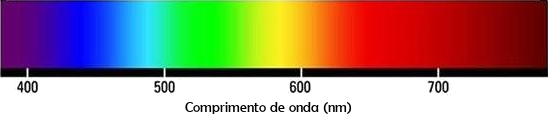
\includegraphics[scale=0.5]{./img/4.png}
						\end{figure}
						\begin{multicols}{3} \begin{itemize}
							\item[$(\red{2})$] Viotela -- Azul
							\item[$(\red{1})$] Ciano -- Verde
							\item[$(\quad)$] Amarelo -- Vermelho
						\end{itemize} \end{multicols}
				\end{itemize}
		
		\item \textbf{Questão 5) (1 ponto)} Exoplanetas podem ser encontrados de 5 formas, mas o mais eficaz até o momento é o \textit{Método de Trânsito}. De maneira simplificada, esse método consiste em detectar a diminuição da luminosidade de uma estrela causada pela passagem do exoplaneta. Para entender melhor como isso acontece, observe o esquema seguinte:
			\begin{figure}[H]
				\centering
				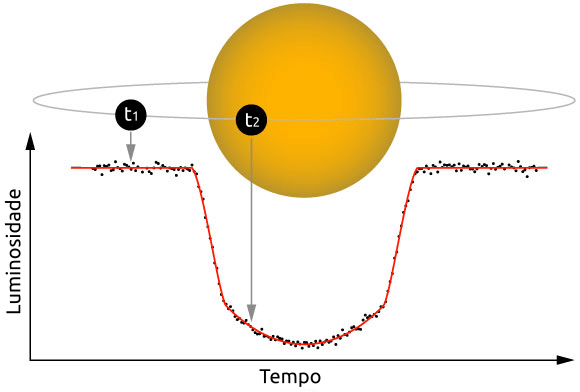
\includegraphics[scale=0.7]{./img/5a.png}
			\end{figure}
			\begin{itemize}
				\item \textbf{Pergunta 5a) (0,5 ponto)} Um problema do \textit{Método de Trânsito} é que a sua eficácia depende da órbita do planeta visualizada. Nesse sentido, marque o(s) exoplaneta(s) abaixo que poderiam ser descobertos por meio desse método.
					\red{\begin{itemize}
						\item Para que um exoplaneta possa ser descoberto pelo \textit{Método de Trânsito}, sua órbita precisa passar em frente a sua estrela.
					\end{itemize}}
					\begin{multicols}{3}
						\begin{figure}[H]
							\centering
							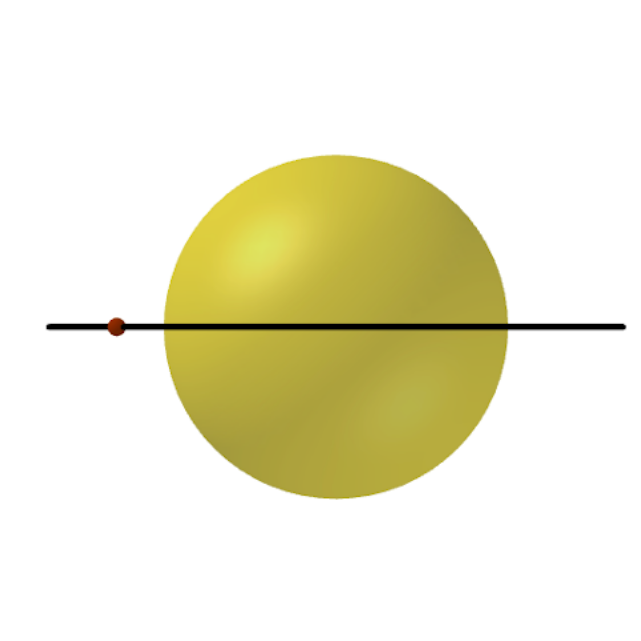
\includegraphics[scale=0.2]{./img/5b1.png}
							\captionsetup{labelformat=empty}
							\caption{$(\red{X})$}
						\end{figure}
						\begin{figure}[H]
							\centering
							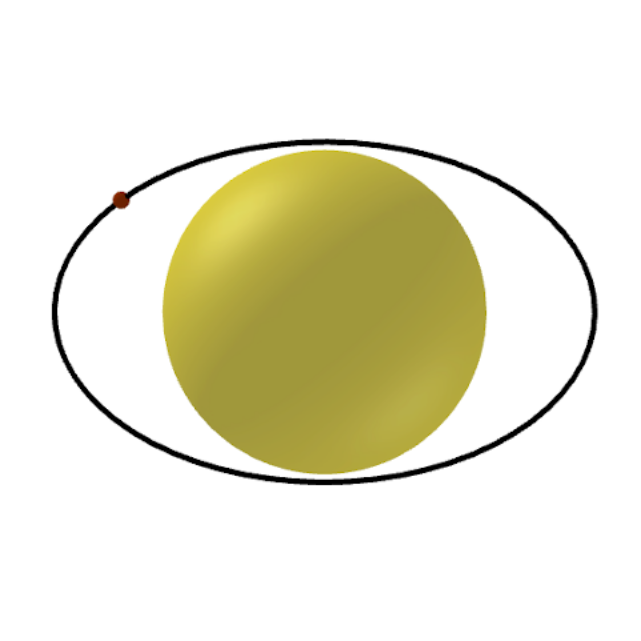
\includegraphics[scale=0.2]{./img/5b2.png}
							\captionsetup{labelformat=empty}
							\caption{$(\quad)$}
						\end{figure}
						\begin{figure}[H]
							\centering
							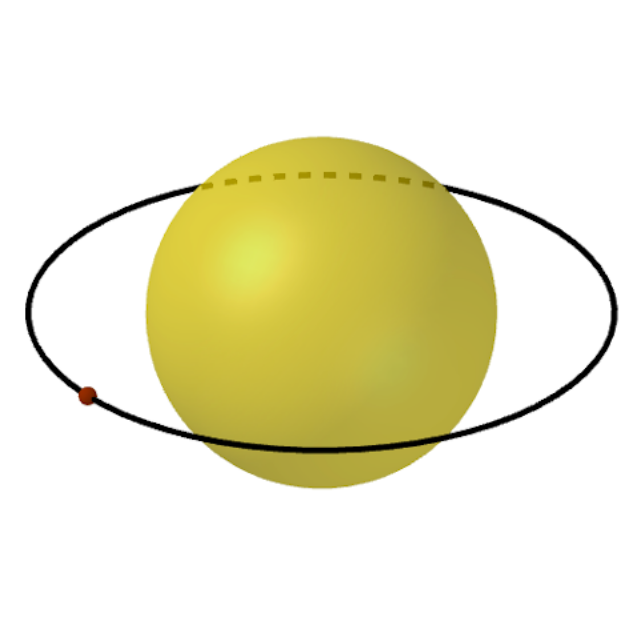
\includegraphics[scale=0.2]{./img/5b3.png}
							\captionsetup{labelformat=empty}
							\caption{$(\red{X})$}
						\end{figure}
						\begin{figure}[H]
							\centering
							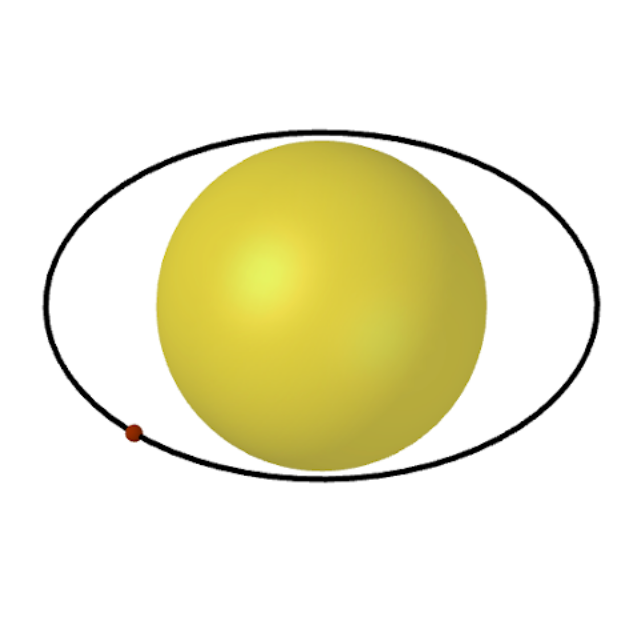
\includegraphics[scale=0.2]{./img/5b4.png}
							\captionsetup{labelformat=empty}
							\caption{$(\quad)$}
						\end{figure}
						\begin{figure}[H]
							\centering
							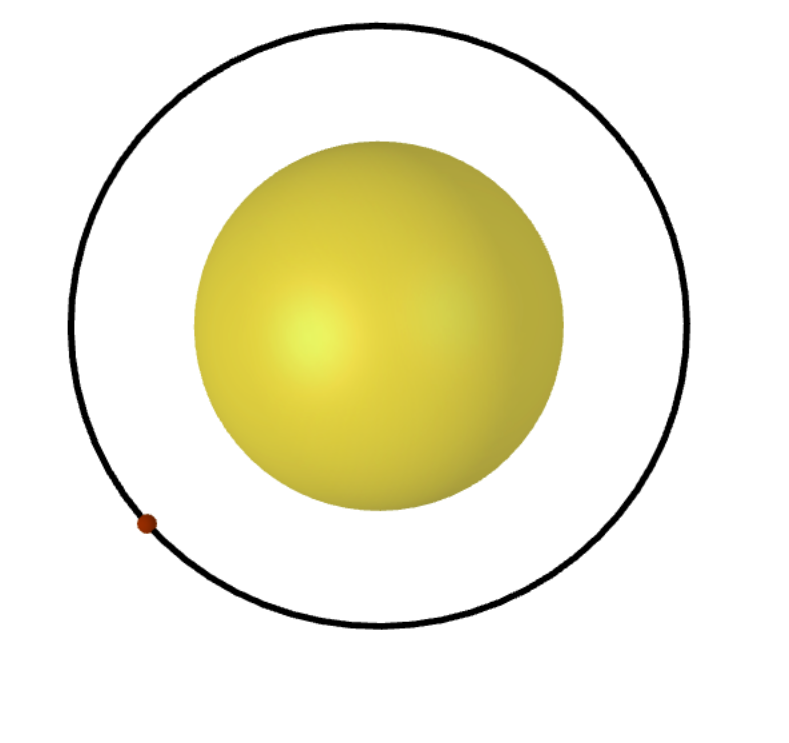
\includegraphics[scale=0.2]{./img/5b5.png}
							\captionsetup{labelformat=empty}
							\caption{$(\quad)$}
						\end{figure}
						\begin{figure}[H]
							\centering
							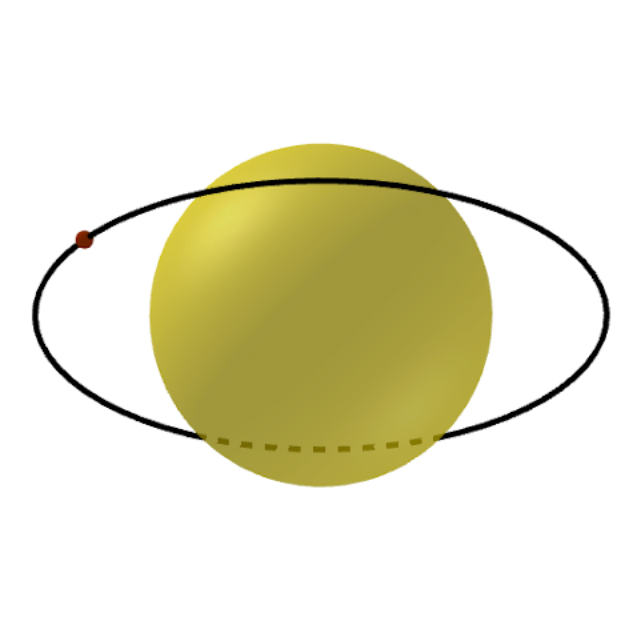
\includegraphics[scale=0.2]{./img/5b6.png}
							\captionsetup{labelformat=empty}
							\caption{$(\red{X})$}
						\end{figure}
					\end{multicols}
				\item \textbf{Pergunta 5b) (0,5 ponto)} Sabendo que $R_e$ e $R_p$ são respectivamente os raios da estrela e do exoplaneta, qual a razão das luminosidades $L_2$ (medida em $t_2$) e $L_1$ (medida em $t_1$)? \linebreak
					\textbf{Dica:} neste caso, podemos usar que a luminosidade é proporcional à área da seção transversal. \linebreak
					\textbf{Espaço para cálculos:}
					\red{\begin{itemize}
						\item A área da seção transversão em $t_1$, é dada por:
							$$At_1 = \pi R_e^2$$
						\item A área da seção transversão em $t_2$, é dada por:
							$$At_2 = \pi (R_e^2-R_p^2)$$
							(basta subtrair a área transversal correspondente ao exoplaneta, $A=\pi R_p^2$, da área transversal correspondente à estrela, $A=A_1=\pi R_e^2$)
						\item Como $L \propto A$, temos:
							$$\frac{L_2}{L_1} = \frac{A_2}{A_1} = \frac{\pi (R_e^2-R_p^2)}{\pi R_e^2}$$
							$$\therefore \quad \frac{L_2}{L_1} = \frac{R_e^2-R_p^2}{R_e^2}$$
					\end{itemize}}
					\begin{multicols}{2} \begin{itemize}
						\item[$(\quad)$] $\frac{L_2}{L_1} = \left( \frac{R_p}{R_e} \right)^2$
						\item[$(\quad)$] $\frac{L_2}{L_1} = \left( \frac{R_e}{R_p} \right)^2 $
						\item[$(\red{X})$] $\frac{L_2}{L_1} = \frac{R_e^2-R_p^2}{R_e^2}$
						\item[$(\quad)$] $\frac{L_2}{L_1} = \frac{R_p^2-R_e^2}{R_p^2}$
					\end{itemize} \end{multicols}
			\end{itemize}
	\end{itemize}
	\end{flushleft}
	\begin{flushright}
		\begin{large}
			Bons estudos!
		\end{large}
	\end{flushright}
\end{document}